\documentclass[a4paper, 10pt]{article}
%encoding
%---------------------------------------------------------
\usepackage[utf8]{inputenc}
\usepackage[T1]{fontenc}
%----------------------------------------------------------------------
\usepackage{geometry}
\geometry{left=3cm,right=3cm,top=2.5cm,bottom=2.5cm}
\usepackage[german]{babel}
\usepackage{amsmath}
\usepackage{amsfonts}
\usepackage{amssymb}
\usepackage{array}
\usepackage{graphicx}
\graphicspath{ {img/} }
\usepackage{hyperref}
\usepackage{listings}
\usepackage{verbatim}
\usepackage[shortlabels]{enumitem}
\usepackage[sorting=none]{biblatex}
\bibliography{refs}

\begin{document}
\renewcommand{\abstractname}{\vspace{-\baselineskip}}

\title{Elite*Shitcoin: Ein elektronisches Peer-to-Peer-Bezahlsystem}
\author{Eduard Nikoleisen \\ 
\href{mailto:eduard.nikoleisen@eddy-dev.net}{eduard.nikoleisen@eddy-dev.net}\\ \url{https://www.justhold.de} \\ \url{https://github.com/Der-Eddy/elite-shitcoin}}
\date{}


\maketitle
\begin{center}
\parbox{0.8\linewidth}{\noindent \textbf{Abstract.} Eine reine Peer-to-Peer-Version eines elektronischen Zahlungsverfahrens würde es ermöglichen, dass Online-Zahlungen von einer Partei direkt an eine andere gesendet werden, ohne über ein Finanzinstitut zu gehen. Digitale Signaturen bilden einen Teil der Lösung, aber die Hauptvorteile gehen verloren, wenn weiterhin eine vertrauenswürdige dritte Partei notwendig ist, um Double Spending (Mehrfachausgaben) zu verhindern. Wir schlagen eine Lösung für das Double-Spending-Problem vor, indem wir ein Peer-to-Peer-Netzwerk benutzen. Das Netzwerk gibt Transaktionen einen Zeitstempel, indem es sie in eine fortlaufende Kette von Hash-basierten Arbeitsbeweisen (Proof-of-Work) hasht und so eine Aufzeichnung erzeugt, die nicht geändert werden kann, ohne den Proof-of-Work neu zu erzeugen. Die längste Kette dient nicht nur als Nachweis für die Sequenz bezeugter Ereignisse, sondern auch als Beweis, dass sie vom größten Pool an CPU-Leistung stammt. Solange der Großteil der CPU-Leistung von Nodes kontrolliert wird, die nicht kooperieren, um das Netzwerk anzugreifen, werden diese die längste Kette generieren und schneller sein als die Angreifer. Das Netzwerk selbst erfordert nur eine Minimalstruktur. Nachrichten werden auf Best-Effort-Basis übertragen und die Nodes können das Netzwerk beliebig verlassen und wieder betreten, da sie die längste Proof-of-Work-Kette als Beweis darüber akzeptieren, was geschah, während sie weg waren. }
\end{center}

\

\section{Einleitung}\label{introduction}

Handel im Internet beruht heutzutage fast ausschließlich darauf Zahlungsverfahren von Finanzinstitute/Banken zu nutzen und auf diese zu vertrauen. Diese Zahlungsverfahren setzen auf Vertrauen und können nicht garantieren das man Transaktion nicht Vollständig unumkehren kann. Außerdem fallen bei den Transaktionen Kosten an in Bezug auf die Vermittlungs zwischen den Finanzinstituten an. Notwendig ist deswegen ein elektronisches Zahlungssystem welches einen kryptographischen Nachweis an Stelle von Vertrauen einsetzt und eine direkte Transaktion zwischen zwei Personen ermöglicht, ohne Mittelsmänner. Transaktionen, bei denen es rechnerisch unmöglich ist, sie zu widerrufen, würden die Verkäufer vor Betrug schützen. Dafür wird ein Hash der letzten Trannsaktionen mit in den neuen Satz/Block an Transaktionen angehängt, Änderungen an einer Transaktionen in der Vergangen würden zu einem exponentiellenl großen Rechenaufwand anwachsen.

\newpage

\section{Transaktionen}\label{transactions}

Inzwischen liest keine Sau mehr das Whitepaper, wenn du dies liest, hast du wahrscheinlich sehr viel Langeweile oder möchtest dich tatsächlich mit einer Kryptowährung auseinandersetzen. 

\begin{figure}[!h]
\centering
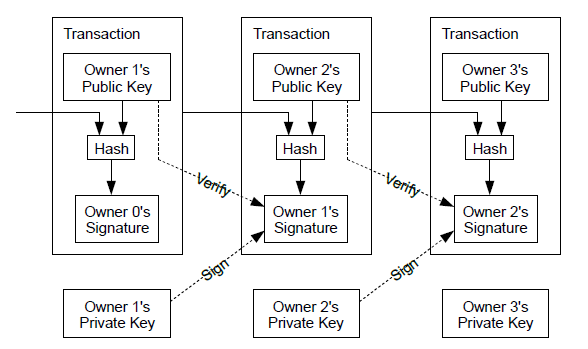
\includegraphics[width=0.75\linewidth]{transactions.png}
\end{figure}

Das Bild oben ist aus dem Original Whitepaper von Satoshi Nakamoto, der Rest von diesem Whitepaper basiert auch lose auf dem Original von Satoshi. Das Bitcoin Whitepaper war damals tatsächlich auch das Erste was ich gelesen habe, danach kam noch das Litecoin Whitepaper und dann sehr lange nichts. Interessant ist auch das man bis heute nicht weiß wer genau unter dem Pseudonym Satoshi Nakamoto eigentlich steckt, man geht davon aus das er Japaner ist, auch wenn es merkwürdig ist das ein Japaner fast ausschließlich auf Englisch geschrieben hat. Seine letzte Aktivität an Bitcoin lässt auf 2010 datieren, seit dem haben andere das Projekt Bitcoin in die Hand genommen. Einer der ersten Nutzer und Entwickler an Bitcoin war auch Hal Finney, er erstellte bereits 2004 ein Proof-of-Work System und hat die erste Transaktion von Bitcoin erhalten. Finney starb 2014 an ALS (Bekannt von der Ice Bucket Challenge). Heute ist es eigentlich schade was mit Bitcoin passiert, die derzeitigen Entwickler verkrüppeln Bitcoin absichtlich um Second-Layer Solutions wie SegWit und Lightning Network nützlicher zu gestalten als sie eigentlich wären. Dennoch gehört Bitcoin zum mit Abstand beliebtesten Kryptowährung trotz den hohen Transaktionsgebühren, welche durch die Verkrüpplung der Entwickler kommt.

\section{Proof-of-Work}\label{proof-of-work}

Proof-of-Work ist auf lange Sicht zum Tode verbannt. Der Wechsel von Ethereum zu PoS (Proof-of-Service) wird der erste große Schritt sein und damit enden das Regierungen das Mining von ineffizienten Kryptowährungen wie z.B. Bitcoin verbieten. Schon heute verbraucht das Bitcoin Mining enormen Abfall an ASIC-Miner die nach einiger Zeit nur nutzloser Schrott sind und verbraucht Strom der ausreicht um ganze Länder zu versorgen. Ob PoS der richtige Schritt ist um Kryptowährungen effizienter zu gestalten, steht noch in den Sternen.

\begin{figure}[!h]
\centering
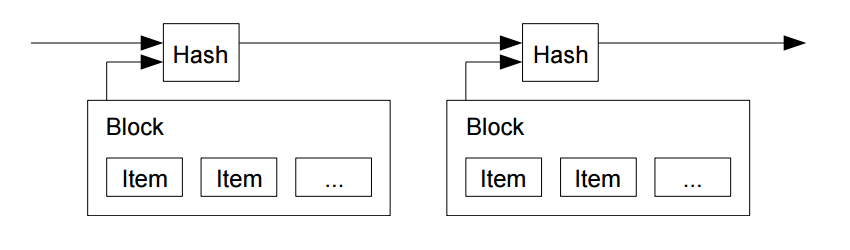
\includegraphics[width=0.75\linewidth]{proof-of-work.png}
\end{figure}
\newpage

\section{Fazit}\label{conclusion}

Glückwunsch, du hast diesen Witz eines Whitepapers bis zum Schluss gelesen oder zumindest bis ans Ende gescrollt. Anzumerken sei das die Token die ich erstellt habe nur aufzeigen soll wie einfach es ist eine nutzlose Token zu erstellen und eine ICO zu vermarkten ist. Der Wert von meiner Token geht gegen Null, ich möchte keinen meckern hören wenn er sein Geld (in Ether) zurück haben möchte.
Original Whitepaper von: https://github.com/karask/satoshi-paper

\newpage

\printbibliography


\end{document}
